\chapter{Metodologia}

La metodología propuesta se organiza en cuatro etapas principales: adquisición y preparación de datos, formulación y entrenamiento de la PINN, diseño experimental de hiperparámetros, y evaluación del modelo entrenado. El propósito central es combinar observaciones dispersas de estaciones meteorológicas con restricciones físicas derivadas de las ecuaciones de Navier-Stokes para estimar variables atmosféricas en puntos no medidos sobre la región Caribe de Colombia.

\section{Datos de entrada}

Los datos provienen del portal de Datos Abiertos Colombia (\url{https://www.datos.gov.co/}), que publica registros históricos del IDEAM. Se utilizó el conjunto de registros de estaciones meteorológicas de la región Caribe correspondientes al mes de diciembre de 2025, cubriendo los departamentos de Atlántico, Bolívar, Magdalena, Sucre y Córdoba. El archivo consolidado contiene 16.368 registros horarios distribuidos en aproximadamente 22 estaciones.

La extensión geográfica del dominio de estudio fue calculada a partir de las coordenadas de las 18 estaciones que integran el conjunto de entrenamiento, una vez aplicados los criterios de exclusión descritos en la sección de preprocesamiento. La latitud varía entre $7{,}4750^{\circ}$\,N y $11{,}1150^{\circ}$\,N, y la longitud entre $76{,}2240^{\circ}$\,O y $73{,}9260^{\circ}$\,O. Aplicando la fórmula de Haversine, la extensión norte–sur es de aproximadamente 404{,}7\,km y la extensión este–oeste de 252{,}2\,km, con una diagonal total del dominio de 476{,}9\,km. La Tabla~\ref{tab:dominio_geografico} resume estas dimensiones.

\begin{table}[H]
\centering
\caption{Extensión geográfica del dominio de estudio}
\label{tab:dominio_geografico}
\begin{tabular}{ll}
\hline
Dimensión & Valor \\
\hline
Latitud mínima & $7{,}4750^{\circ}$ N \\
Latitud máxima & $11{,}1150^{\circ}$ N \\
Longitud mínima & $76{,}2240^{\circ}$ O \\
Longitud máxima & $73{,}9260^{\circ}$ O \\
Extensión N--S & 404{,}7 km \\
Extensión E--O & 252{,}2 km \\
Diagonal del dominio & 476{,}9 km \\
Resolución de malla (barrido) & $R = 0{,}1^{\circ}$ ($\approx$ 11{,}1 km) \\
Latitud media del centroide & $9{,}295^{\circ}$ N \\
\hline
\end{tabular}
\end{table}

Las estaciones se concentran en la franja costera de los cinco departamentos analizados; la extensión este–oeste (252{,}2\,km) es notablemente menor que la extensión norte–sur (404{,}7\,km), lo que refleja la distribución lineal de la red de observación a lo largo del litoral. Las zonas del interior continental y la franja marítima carecen de cobertura directa, lo que refuerza la motivación del enfoque propuesto.

Cada observación incluye las siguientes variables:

\begin{itemize}
	\item Identificador y posición geográfica de la estación (latitud, longitud, altitud).
	\item Marca temporal expresada en segundos desde el inicio del periodo.
	\item Velocidad del viento (m/s) y dirección del viento (grados).
	\item Presión atmosférica (mbar).
	\item Temperatura del aire (°C).
\end{itemize}

\subsection{Caracterizacion descriptiva inicial del conjunto}

Como apoyo a la descripcion de los datos de entrada, la Figura~\ref{fig:serie_temporal_datos_caribe} resume el comportamiento temporal de las variables registradas durante el periodo de estudio. Esta evidencia visual permite identificar variabilidad intraperiodo y cambios de escala entre variables, aspectos que motivan las etapas de preprocesamiento y escalamiento descritas en las subsecciones siguientes.

% IMAGEN PENDIENTE: docs/descripcion_datos/em_caribe_time_series.png
% \begin{figure}[H]
% \centering
% 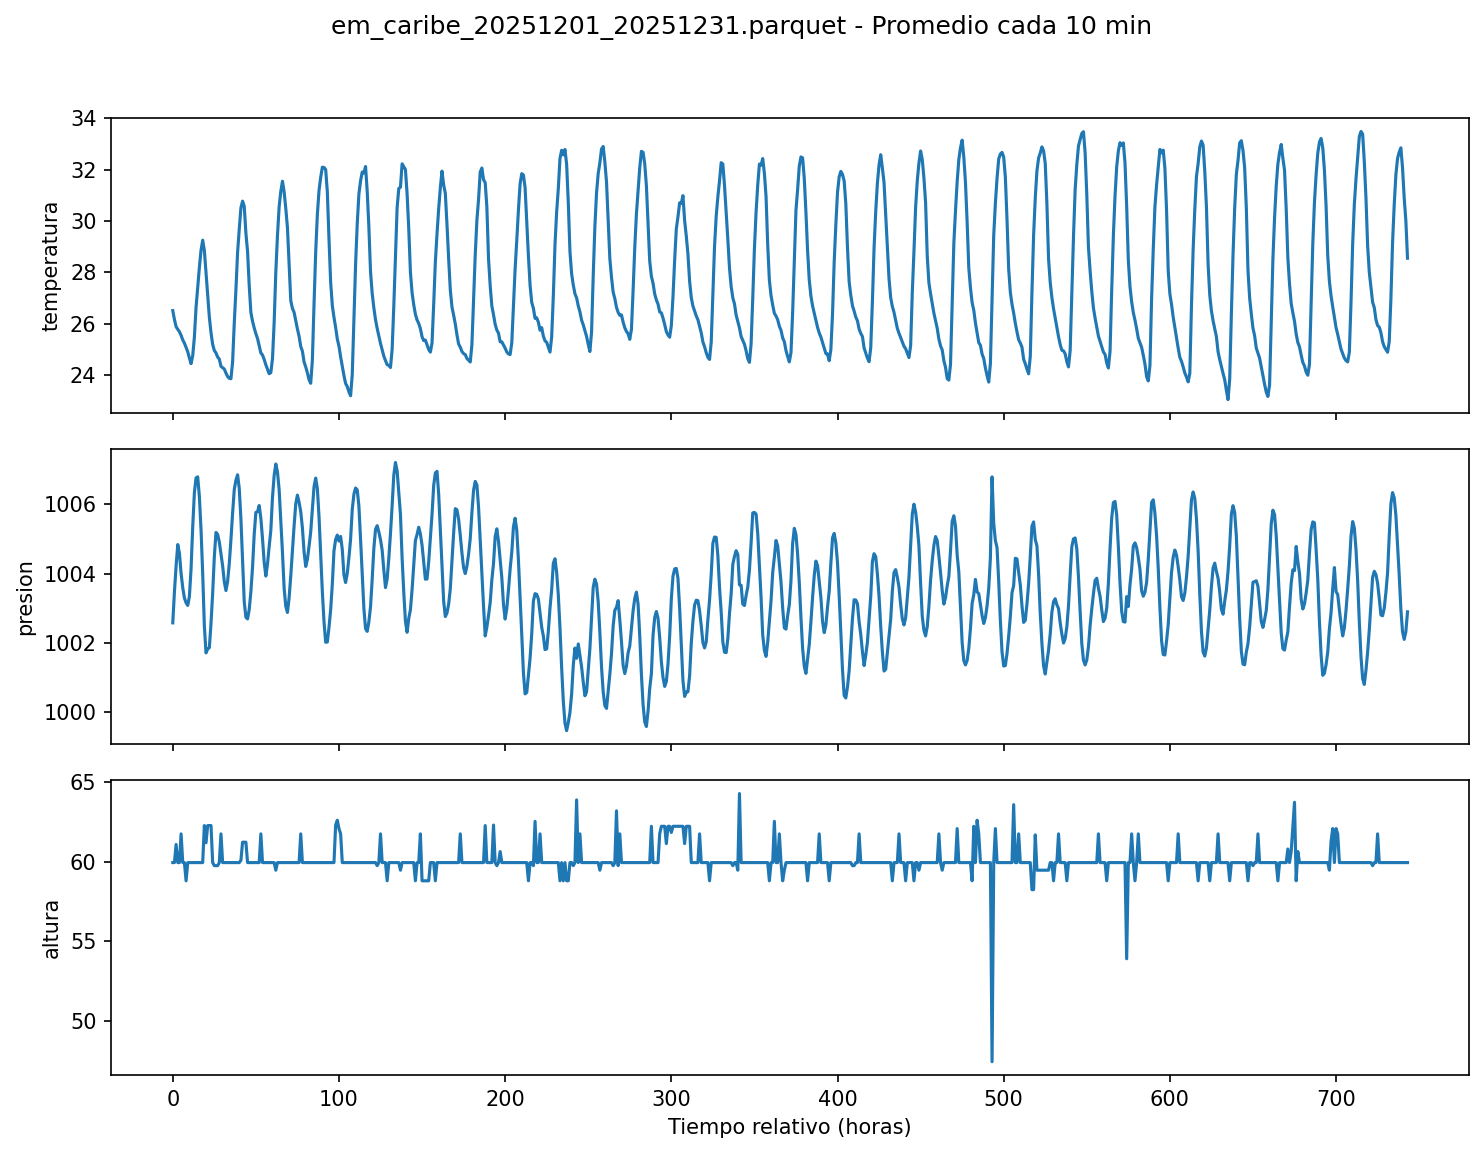
\includegraphics[width=0.95\textwidth]{docs/descripcion_datos/em_caribe_time_series.png}
% \caption{Serie temporal descriptiva de variables meteorologicas del conjunto Caribe para diciembre de 2025. La figura se incorpora como evidencia exploratoria del comportamiento temporal previo al entrenamiento de la PINN.}
% \label{fig:serie_temporal_datos_caribe}
% \end{figure}

\section{Preprocesamiento de la información}

El pipeline de preprocesamiento ejecuta las siguientes etapas en secuencia:

\subsection{Selección y exclusión de estaciones}

Se excluyen cuatro estaciones que presentan anomalías críticas en presión o en las componentes de viento. La Tabla~\ref{tab:estaciones_excluidas} detalla los criterios de exclusión aplicados. Tras la exclusión, se retienen 18 estaciones válidas, distribuidas geográficamente a lo largo de los cinco departamentos del área de estudio, como se ilustra en la Figura~\ref{fig:mapa_estaciones}.

\begin{table}[H]
\centering
\caption{Estaciones excluidas y criterio de exclusión aplicado}
\label{tab:estaciones_excluidas}
\begin{tabular}{lll}
\hline
Código de estación & Anomalía detectada        & Variable afectada \\\\
\hline
0025025380         & Presión anómalamente alta & $p$               \\\\
0025025030         & Error elevado             & $u_x$             \\\\
0025025190         & Error elevado             & $u_x$             \\\\
0015015100         & Error elevado             & $u_x$             \\\\
\hline
\end{tabular}
\end{table}

En el barrido de hiperparámetros se seleccionan los primeros 300 registros por estación, ordenados cronológicamente, lo que produce un subconjunto rectangular de $18 \times 300 = 5\,400$ registros. Una corrida adicional posterior utilizó la totalidad de los registros disponibles ($18 \times 744 = 13\,392$ registros) con la configuración óptima.

\begin{figure}[H]
\centering
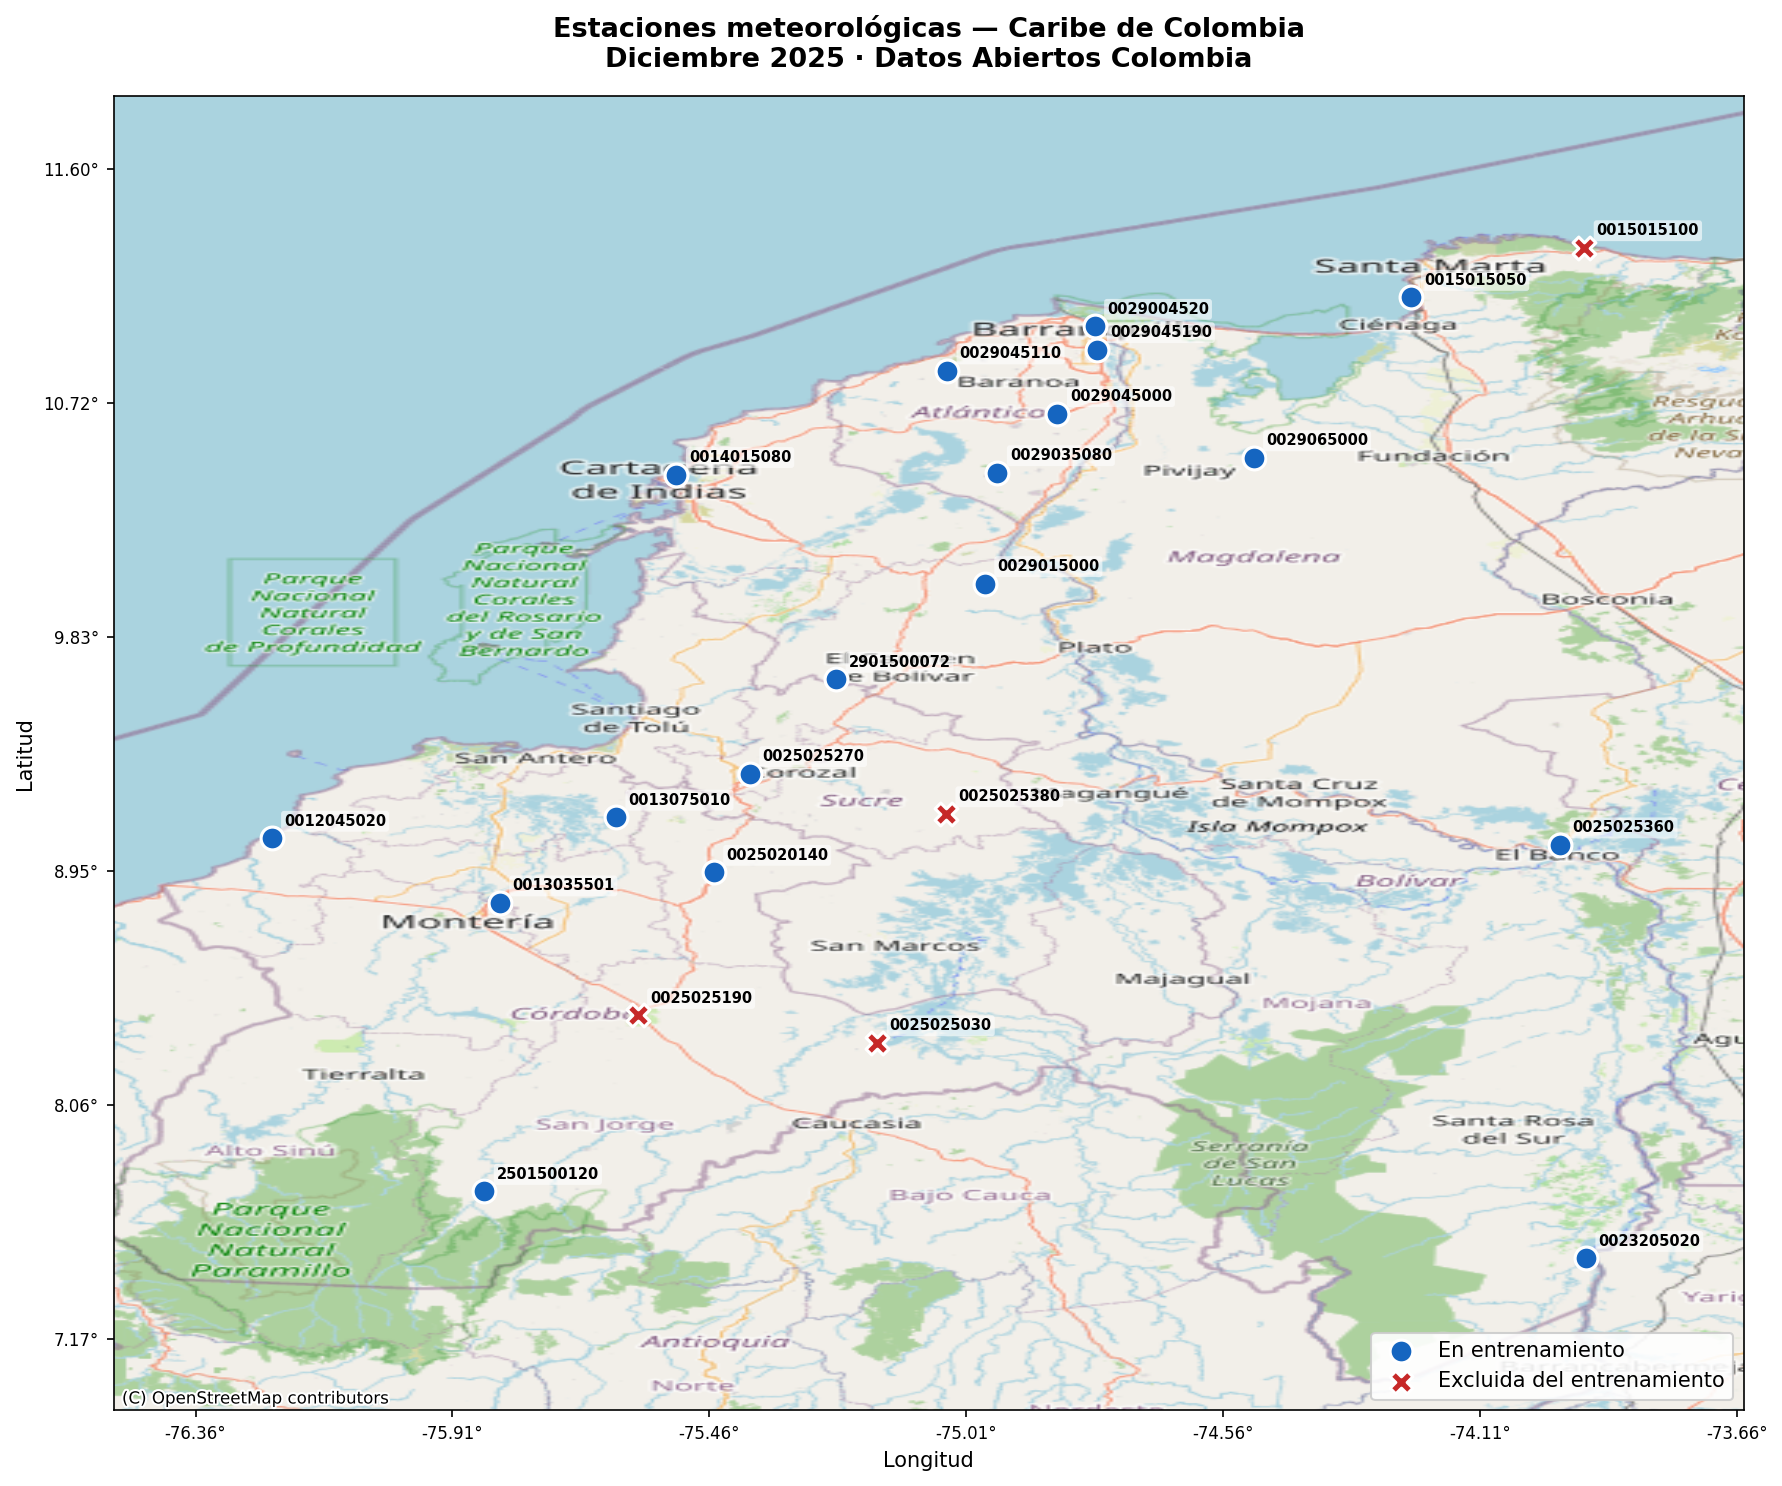
\includegraphics[width=0.85\textwidth]{Imagenes/mapa_estaciones_caribe.png}
\caption{Distribución geográfica de las estaciones meteorológicas del IDEAM en la región Caribe de Colombia. Los marcadores azules corresponden a las 18 estaciones válidas incluidas en el entrenamiento; los marcadores rojos identifican las 4 estaciones excluidas por anomalías en presión o en las componentes de viento.}
\label{fig:mapa_estaciones}
\end{figure}

\subsection{Descomposición del viento y proyección cartesiana}

La velocidad y la dirección del viento se descomponen en componentes cartesianas $u_x$ (componente Este–Oeste) y $u_y$ (componente Norte–Sur). Las coordenadas geográficas (latitud $\varphi$, longitud $\lambda$) se convierten a distancias en metros mediante aproximación de arco de círculo con radio terrestre $R_T = 6\,378\,000\,\text{m}$. Sea $(x_c, y_c)$ el centroide geográfico del dominio; entonces:

\[
x_i = R_T \cdot \sin\left(\frac{\pi}{180}\,\Delta\lambda_i\right), \qquad y_i = R_T \cdot \sin\left(\frac{\pi}{180}\,\Delta\varphi_i\right)
\]

donde $\Delta\lambda_i$ y $\Delta\varphi_i$ son los desplazamientos angulares respecto al centroide. Esta transformación produce un dominio cartesiano localizado en la región Caribe, con origen en el centroide. Las unidades resultantes son metros.

\subsection{Corrección de presión al nivel del mar}

La presión medida en cada estación se corrige al nivel del mar usando el modelo de atmósfera estándar internacional (ISA):

\[
P_{\text{corr}} = P \cdot \left(1 - \frac{0{,}0065 \cdot Z}{T + 273{,}15 + 0{,}0065 \cdot Z}\right)^{-5{,}257}
\]

donde $Z$ es la altitud de la estación en metros y $T$ es la temperatura en °C.

\subsection{Adimensionalización}

Todas las variables se adimensionalizan antes del entrenamiento para que la red opere con magnitudes comparables. Las escalas de referencia se calculan a partir de los propios datos:

\begin{itemize}
	\item $L$: rango máximo entre desplazamientos en $x$ o $y$ (escala de longitud).
	\item $W$: escala de velocidad observada, calculada a partir de los datos de viento.
	\item $\rho W^2$: presión dinámica de referencia (escala de presión).
	\item $T$: horizonte temporal total del período de estudio ($T = N_{\text{DIAS}} \cdot 86\,400\,\text{s}$).
\end{itemize}

Las transformaciones aplicadas son:

\[
x_{\text{norm}} = \frac{x}{L}, \quad y_{\text{norm}} = \frac{y}{L}, \quad t_{\text{norm}} = \frac{t}{T}
\]
\[
u_{\text{norm}} = \frac{u_x}{W}, \quad v_{\text{norm}} = \frac{u_y}{W}, \quad p_{\text{norm}} = \frac{p}{\rho W^2}
\]

El reescalado de presión por su desviación estándar ($\sigma_p = 1{,}9656$) representa una corrección adicional para equilibrar el rango de la presión normalizada con el de las velocidades, reduciendo asimetría numérica en la función de pérdida combinada.

\section{Definición de entradas y salidas del modelo}

La PINN recibe tres variables de entrada:
\[
(x, y, t)
\]
donde $x$ e $y$ representan la posición espacial normalizada y $t$ el tiempo normalizado. A partir de estas entradas, la red produce tres salidas:
\[
(vel_u,\ vel_v,\ p)
\]
correspondientes a las componentes cartesianas del viento y la presión, todas en escala adimensional.

\section{Arquitectura de la red}

La red neuronal implementa la capa \texttt{GammaBiasLayer}, una extensión de la capa lineal estándar que incorpora \textit{Weight Normalization} desacoplada y parámetros $\gamma$ (escalado) y $\beta$ (desplazamiento) entrenables. La transformación de cada capa es:

\[
y = \gamma \cdot \left(\hat{W}\,x\right) + \beta, \qquad \hat{W} = \frac{W}{\|W\|}
\]

La estructura completa de la red es:

\begin{table}[H]
\centering
\begin{tabular}{lllll}
\hline
Capa & Tipo & Activación & Dim. entrada & Dim. salida \\
\hline
Entrada & GammaBiasLayer & Tanh & 3 & 1.200 \\
Ocultas 1–7 & GammaBiasLayer & Tanh & 1.200 & 1.200 \\
Ocultas 8–11 & GammaBiasLayer & Lineal & 1.200 & 1.200 \\
Salida & GammaBiasLayer & — & 1.200 & 3 \\
\hline
\end{tabular}
\caption{Estructura de la red PINN para predicción meteorológica en el Caribe. Total de parámetros entrenables: 15.890.409.}
\label{tab:arquitectura_pinn}
\end{table}

La arquitectura seleccionada consta de 12 capas con 1.200 neuronas por capa, totalizando aproximadamente 15{,}89 millones de parámetros entrenables para 13.392 puntos de entrenamiento (ratio $\approx$ 1.186:1). Esta elección se sustenta en dos consideraciones. En primer lugar, las PINNs de alta capacidad expresiva han mostrado ventajas en problemas de predicción de campos continuos con restricciones diferenciales \citep{raissi2019physics}, donde la red debe aproximar funciones suaves sobre todo el dominio y no únicamente en los puntos de observación. En segundo lugar, la pérdida física evaluada sobre los 226.176 puntos de colocación actúa como regularizador implícito, reduciendo el riesgo de sobreajuste que normalmente se asocia con redes sobredimensionadas en el aprendizaje supervisado puro. Nótese que el trabajo original de PINNs \citep{raissi2019physics} utilizó redes de 4--8 capas con 20--100 neuronas, significativamente más pequeñas; la escala del dominio meteorológico estudiado aquí justifica una red de mayor capacidad, aunque la evaluación de configuraciones reducidas queda propuesta como experimento de ablación en trabajos futuros.

La combinación de capas Tanh (primeras 8 capas) y capas lineales finales (últimas 4 capas) actúa como mecanismo de regularización implícita por construcción, facilitando la convergencia del modelo hacia soluciones suaves y físicamente consistentes.

\section{Ecuaciones físicas: Navier-Stokes invíscido}

El residual físico se calcula mediante diferenciación automática sobre las predicciones de la red. Se implementan las ecuaciones de Euler incompresible bidimensionales en dominio adimensionalizado:

\textbf{Ecuación de continuidad:}
\[
\frac{\partial u_x}{\partial x} + \frac{\partial u_y}{\partial y} = 0
\]

\textbf{Momento en $x$:}
\[
\frac{\partial u_x}{\partial t} + u_x \frac{\partial u_x}{\partial x} + u_y \frac{\partial u_x}{\partial y} + \frac{\partial p}{\partial x} = 0
\]

\textbf{Momento en $y$:}
\[
\frac{\partial u_y}{\partial t} + u_x \frac{\partial u_y}{\partial x} + u_y \frac{\partial u_y}{\partial y} + \frac{\partial p}{\partial y} = 0
\]
\subsection{Justificación de la omisión del término de Coriolis}

Las ecuaciones implementadas no incluyen el término de Coriolis $(-f \times \mathbf{u})$, donde $f = 2\Omega\sin(\varphi)$ es el parámetro de Coriolis, $\Omega = 7{,}2921 \times 10^{-5}\,\text{rad/s}$ es la velocidad angular de rotación terrestre y $\varphi$ es la latitud. Para la latitud media del dominio ($\varphi_{\text{medio}} = 9{,}295^{\circ}\,\text{N}$), este parámetro toma el valor $f = 2{,}3556 \times 10^{-5}\,\text{s}^{-1}$.

La relevancia relativa del término de Coriolis frente a las fuerzas de inercia se cuantifica mediante el número de Rossby:
\[
Ro = \frac{W}{f \cdot L}
\]
donde $W$ es la velocidad característica del flujo y $L$ la escala de longitud del dominio. Con $W = 10{,}80\,\text{m/s}$ (velocidad de referencia de normalización del modelo) y $L = 476{,}9\,\text{km}$ (diagonal del dominio, Tabla~\ref{tab:dominio_geografico}), se obtiene $Ro = 0{,}96$.

Un número de Rossby cercano a la unidad indica que los efectos de inercia y los efectos de Coriolis son comparables en magnitud, lo que corresponde a un régimen de transición geostrófica. Esto implica que la omisión del término de Coriolis en las ecuaciones implementadas constituye una simplificación metodológica significativa: a la escala del Caribe colombiano (diagonal $\approx$ 477\,km), el balance geostrófico entre el gradiente de presión y la fuerza de Coriolis es un mecanismo dinámico relevante. La omisión de este término tiende a subestimar la curvatura de las trayectorias del viento y el acoplamiento entre el campo de presiones y el campo de velocidades a escala sinóptica. Esta limitación se declara explícitamente y su incorporación se propone como extensión del modelo en trabajos futuros.
El residual de Navier-Stokes se evalúa tanto en los puntos de las estaciones como en los puntos de la malla de colocación, garantizando la satisfacción de la física en todo el dominio, incluyendo zonas sin observaciones.

\section{Formulación de la función de pérdida}

La red se entrena mediante una función de pérdida compuesta por cuatro términos:

\[
\mathcal{L}_{\text{total}} = \lambda \cdot \mathcal{L}_{\text{NS}}^2 + \mathcal{L}_{u_x}^2 + \mathcal{L}_{u_y}^2 + \mathcal{L}_p^2
\]

donde cada término es el error cuadrático medio sobre el batch correspondiente:

\[
\mathcal{L}_{u_x} = \frac{1}{N}\sum_{i=1}^N \left(\hat{u}_{x,i} - u_{x,i}^{\text{obs}}\right)^2
\]

El término $\mathcal{L}_{\text{NS}}$ incorpora el residuo de las ecuaciones de Euler, evaluado sobre los puntos de colocación:

\[
\mathcal{L}_{\text{NS}} = \text{MSE}(e_{\text{cont}}, 0) + \text{MSE}(e_{\text{mom}_x}, 0) + \text{MSE}(e_{\text{mom}_y}, 0)
\]

El hiperparámetro $\lambda$ controla el balance entre fidelidad a las observaciones (los tres primeros términos) y cumplimiento de las restricciones físicas (el término ponderado por $\lambda$).

Como extension metodologica posterior al barrido base, se implemento una variante de la funcion de perdida con restriccion suave de rango para controlar predicciones fisicamente inverosimiles en zonas sin observacion directa. En esta variante se calcularon limites robustos por variable a partir de los cuantiles $Q_{0.01}$ y $Q_{0.99}$ del conjunto de entrenamiento, y se penalizaron las salidas fuera de ese intervalo mediante una funcion softplus diferenciable.

Para una variable $k \in \{u_x, u_y, p\}$, los limites de rango se definieron como:

\[
l_k^- = Q_{0.01}(y_k), \qquad l_k^+ = Q_{0.99}(y_k)
\]

La penalizacion elemental para una prediccion $\hat{y}_k$ se expreso como:

\[
\mathcal{P}(\hat{y}_k, \tau) =
\tau \ln\!\left(1 + e^{(\hat{y}_k-l_k^+)/\tau}\right)
+
\tau \ln\!\left(1 + e^{(l_k^- - \hat{y}_k)/\tau}\right)
\]

y la perdida de rango total como:

\[
\mathcal{L}^{\text{rango}} = \lambda_R \left(\mathcal{L}^{\text{rango}}_{u_x} + \mathcal{L}^{\text{rango}}_{u_y} + \mathcal{L}^{\text{rango}}_{p}\right)
\]

En esta extension, el peso $\lambda_R$ no se activo de manera abrupta sino mediante una rampa lineal durante las primeras 300 epocas, hasta alcanzar $\lambda_{R,\max}=0{,}50$. La funcion de perdida extendida se definio como:

\[
\mathcal{L}_{\text{total}}^{\text{ext}} =
\frac{\mathcal{L}_{NS}^2 + \mathcal{L}_{u_x}^2 + \mathcal{L}_{u_y}^2 + \mathcal{L}_{p}^2 + \left(\mathcal{L}^{\text{rango}}\right)^2}
{\mathcal{L}_{NS} + \mathcal{L}_{u_x} + \mathcal{L}_{u_y} + \mathcal{L}_{p} + \mathcal{L}^{\text{rango}} + \varepsilon}
\]

donde $\varepsilon = 10^{-12}$ es un termino de estabilidad numerica. Esta formulacion actua como un normalizador dinamico entre los componentes observacionales, fisicos y de rango.

\section{Construcción de la malla espacio-temporal}

Los puntos de colocación donde se evalúa el residuo físico se generan sobre una malla regular definida por la resolución $R$ en grados geográficos. Cada resolución se convierte a metros mediante:

\[
R_{\text{PINN}} = R_T \cdot \sin\left(\frac{\pi}{180}\,R_{\text{grados}}\right)
\]

La malla se extiende $R_{\text{PINN}}$ más allá de los límites de las estaciones en cada dirección. Las resoluciones evaluadas en el barrido de hiperparámetros fueron:

\begin{table}[H]
\centering
\begin{tabular}{lll}
\hline
$R$ (grados) & $N_{\text{espacial}}$ & $N_{\text{colocación total}}$ \\
\hline
0,1 & 304 & 226.176 (300 pasos temporales) \\
0,4 & 44 & 32.736 (300 pasos temporales) \\
\hline
\end{tabular}
\caption{Configuraciones de malla de colocación evaluadas. La dimensión temporal se fija en 300 pasos para el barrido de hiperparámetros.}
\label{tab:malla_coloc}
\end{table}

Todos los puntos espaciales se replican para cada paso temporal, resultando en $N_{\text{colocación}} = N_{\text{espacial}} \times N_{\text{temporal}}$. Una corrida posterior utilizó la totalidad de los 744 pasos temporales disponibles en diciembre de 2025.

\section{Entrenamiento}

El entrenamiento se realiza durante 2.000 épocas con el optimizador Adam utilizando los siguientes hiperparámetros:

\begin{itemize}
	\item Tasa de aprendizaje inicial: $\eta_0 = 1 \times 10^{-4}$
	\item Scheduler: ReduceLROnPlateau con factor de reducción $\alpha = 0{,}3162$ y paciencia de 50 épocas
	\item Recorte de gradiente (gradient clipping): norma máxima $\|g\|_{\max} = 0{,}5$
	\item Hardware: GPU con CUDA, framework PyTorch
\end{itemize}

Se guardan checkpoints en las épocas 500, 1.000, 1.500 y 2.000. La configuración de entrenamiento fue idéntica para todas las corridas del barrido de hiperparámetros, variando únicamente $\lambda$ y $R$.

\section{Diseño experimental: barrido de hiperparámetros}

Con el fin de estudiar el efecto de la resolución de la malla de colocación y del peso de la restricción física sobre el desempeño del modelo, se ejecutó un barrido sistemático de hiperparámetros. Las variables manipuladas fueron:

\begin{itemize}
	\item \textbf{Resolución de malla:} $R \in \{0{,}1^{\circ},\ 0{,}4^{\circ}\}$
	\item \textbf{Peso de la restricción física:} $\lambda \in \{1,\ 3,\ 5,\ 10\}$ para $R = 0{,}1^{\circ}$ y para $R = 0{,}4^{\circ}$
	\item \textbf{Volumen de datos:} 300 registros por estación (subconjunto rectangular $18 \times 300$)
	\item \textbf{Configuración de entrenamiento:} fija para todas las corridas (Adam, ReduceLROnPlateau, gradient clipping)
\end{itemize}

Cada combinación constituyó una corrida independiente con su propio manifiesto de experimento, registrando los parámetros utilizados, las estaciones incluidas y el subconjunto de datos. La convención de nombres adoptada fue \nolinkurl{PINN_caribe_excl4_300xest_R{R}_L{lambda}}.

Posteriormente, se ejecutó una corrida adicional replicando la configuración óptima identificada en el barrido (R = 0,1°, $\lambda = 5$) pero utilizando la totalidad de los registros disponibles (13.392 registros, aproximadamente 744 registros por estación). Esta corrida se denominó \nolinkurl{PINN_caribe_excl4_todos_R01_L5}.

Como extension metodologica adicional, se ejecuto una corrida sobre esa misma configuracion optima con el mecanismo de restriccion suave de rango activado. Esta corrida se denomino \nolinkurl{PINN_caribe_excl4_todosreg_R01_L5_rangeL05} y utilizo $\lambda_{R,\max}=0{,}50$, rampa lineal de 300 epocas, temperatura $\tau=0{,}05$ y limites robustos de rango definidos por los cuantiles 1\% y 99\%.

\section{Criterios de evaluación}

El desempeño de cada corrida se cuantifica mediante dos grupos de métricas, ambas evaluadas sobre los puntos de estación en la época 2.000:

\begin{itemize}
	\item \textbf{Métricas observacionales:} error cuadrático medio sobre las componentes de viento ($\text{MSE}_{u_x}$, $\text{MSE}_{u_y}$) y sobre la presión ($\text{MSE}_p$), en escala adimensional. El error observacional promedio se define como:
	\[
	\overline{\text{MSE}}_{\text{obs}} = \frac{\text{MSE}_{u_x} + \text{MSE}_{u_y} + \text{MSE}_p}{3}
	\]
	
	\item \textbf{Residuo físico:} valor medio del residuo de las ecuaciones de Navier-Stokes sobre los puntos de colocación, denotado $\mathcal{R}_{\text{NS}}$. Este indicador mide el grado en que las predicciones del modelo satisfacen las ecuaciones de Euler incompresible en zonas sin observaciones directas.

	\item \textbf{Fraccion Fuera de Rango (FOR):} metrica diagnostica calculada para cada variable de salida, definida como la proporcion de predicciones fuera del intervalo robusto $[l_k^-, l_k^+]$:
	\[
	\text{FOR}_k = \frac{1}{N}\sum_{i=1}^{N} \mathbf{1}\!\left[\hat{y}_{k,i} < l_k^- \;\vee\; \hat{y}_{k,i} > l_k^+\right]
	\]
	Esta metrica no participa en el gradiente de entrenamiento y se utiliza unicamente para diagnosticar el comportamiento del mecanismo de restriccion de rango sobre el dominio completo de colocacion.
\end{itemize}

Las métricas se generan automáticamente mediante el script \texttt{evaluar.py} a partir de los checkpoints guardados en las épocas señaladas. Los resultados de todas las corridas se registran en archivos JSON con nomenclatura \texttt{metricas\_PINN\_*\_epoca\_2000.json} para facilitar comparación y reproducibilidad.





